\section{Wahrscheinlichkeitsverteilung}

	\subsection{Verteilungsfunktion \skript{77}}
		\begin{tabular}[]{|l|l|}
        	\hline
        	\textbf{diskret} & \textbf{kontinuierlich}\\
        	\hline
        	\hline
        	$P(X\leq x)=F(x)=\sum\limits_{k=-\infty}^x p_k$ &
        	$P(X\leq x)=F(x)=\int\limits_{-\infty}^x
        	\varphi(\tilde{x})d\tilde{x}$\\
  			$P(X>x)=1-P(X\leq x)$ & $P(X>x)=1-P(X\leq x)$\\        	
        	$P(a \le X \leq b)=F(b)-F(a)=\sum\limits_{k=a}^b p_k$ &
  			$P(a \le X \leq b)=F(b)-F(a)=\int \limits_a^b
  			\varphi(\tilde{x})d\tilde{x}$\\
        	\hline
        \end{tabular}

		\subsubsection{Eigenschaften}
  				$$\boxed{\mathbb{D}(F) = \mathbb{R}} \qquad \boxed{\mathbb{W}(F)
  				\in[0,1]} \qquad \boxed{F(-\infty)=0} \qquad  \boxed{F(\infty)=1}
  				\qquad \boxed{F(x) \text{ ist monoton steigend}}$$

\hrule

\subsection{Wahrscheinlichkeitsdichte}
\begin{multicols}{2}
\textbf{Dichtefunktion oder Wahrscheinlichkeitsdichte:} \\
$\varphi(x) = F'(x)$ \\
\textbf{Bei Sprungstellen von F(x):} \\
$\varphi(x) = $ Dirac mit Gewichtung der Sprunghöhe

\columnbreak

	\textbf{Erwartungswert} \\
	\begin{tabular}{l l l}
		$E(\textcolor{red}{X})$ & $ = \int \textcolor{red}{x} \cdot \varphi(x) dx$  & bzw. $\sum \textcolor{red}{x} \cdot p_k$\\
		$E(\textcolor{red}{X^2})$ & $ = \int \textcolor{red}{x^2} \cdot \varphi(x) dx$ & bzw. $\sum \textcolor{red}{x^2} \cdot p_k$\\
		$E(\textcolor{red}{X^N})$ & $ = \int \textcolor{red}{x^N} \cdot \varphi(x) dx$ & bzw. $\sum \textcolor{red}{x^N} \cdot p_k$
	\end{tabular}
\end{multicols}

\hrule

	\subsection{Rechenregeln für $\varphi$ und $F$ \skript{86}}
		\begin{minipage}{11cm}
			\begin{tabular}{ll}
        	\textbf{Gegeben:} &X, Y Zufallsvariablen und $\varphi_X$, $\varphi_Y$
        	bekannt\\
        	\end{tabular}
 
        	\begin{tabular}{p{6cm}p{6cm}}
        	\textbf{Verteilungsfunktion:} & \textbf{Dichte:}\\
        	$F_{X+a}(x)=F_X(x-a)$  &$\varphi_{X+a}(x)=\varphi_X(x-a)$\\
        	$F_{\lambda X}(x)=F_X(\frac{x}{\lambda})$ &$\varphi_{\lambda
        	X}(x)=\varphi_X(\frac{x}{\lambda})\frac{1}{\lambda}$\\
        	$F_{X+Y}(x)=F_X\ast\varphi_Y(y)=F_Y\ast\varphi_X(x)$ &
        	$\varphi_{X+Y}(x)=\varphi_X\ast\varphi_Y(x)$\\
        	$F_{\sqrt{X}}(x)=F_X(x^2)$ &
        	$\varphi_{\sqrt{X}}(x)=2x\varphi_X(x^2)$\\
        	$F_{X^2}(x)=F_X(\sqrt{x})$ &
        	$\varphi_{X^2}(x)=\frac{1}{2}x^{-\frac{1}{2}}\varphi_X(\sqrt{x})$
        	\end{tabular}
		\end{minipage}
		\begin{minipage}{7cm}
        	\subsubsection{Algorithmus Bsp.}
        	\begin{tabular}{ll}
        	1. Definition von $F$ anwenden: $F_{\lambda X}(x)=P(\underbrace
        	{\lambda X\leq x}_{*})$\\ 
        	2. Bedingung * umformen: $P(X \leq
        	\frac{x}{\lambda})=F_X(\frac{x}{\lambda})$\\ 
        	3. für Dichte: $\frac{d}{dx}$\\
        	\vspace{3mm}
        	$\varphi_{\lambda X}(x)=\frac{d}{dx}F_{\lambda
        	X}(x)=\frac{d}{dx}F_X(\frac{x}{\lambda})=
        	\varphi_X(\frac{x}{\lambda})\frac{1}{\lambda}$
        	\end{tabular}
			\vspace{10mm}
        \end{minipage}
        \subsubsection{Maximalwert eines Intervalls \skript{125}}
		$X_1,\ldots X_i$ sind auf dem Intervall $[0,l]$ mit $F_X(x)$ verteilt\\
		M=$\max \{ X_1,\ldots,X_i\} $ \\
		$F_M(x)=F_X(x)^n$ \\

\newpage

	\subsection{Normalverteilung \skript{101}}
		\begin{floatingfigure}[r]{8cm}
		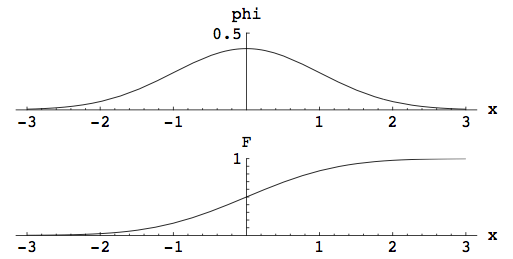
\includegraphics[width=8cm]{./bilder/normalverteilung.png}
		\caption{Dichtefunktion (oben) und Verteilungsfunktion (unten) der
		Normalverteilung.}
   		\end{floatingfigure}
		Viele kleine, unabhängige Zufallsvariable sammeln sich zu einer
		normalverteilten Zufallsvariable.\\
		 $\varphi(x)=\frac{1}{\sqrt{2
		\pi}\sigma}\cdot e^{-\frac{(x-\mu)^2}{2\sigma^2}} = N(\mu ; \sigma) $\\ 
		$F(x)=\frac{1}{\sqrt{2
		\pi}\sigma}\cdot \int\limits^{x}_{-\infty}{e^{-\frac{(\tilde{x} -\mu)^2}{2\sigma^2}}} $ \\
		Addieren von Normalverteilungen: \\
		\fbox{$N(\mu_{1} ; \sigma_{1}) + N(\mu_{2} ; \sigma_{2})
		= N(\mu_{1} + \mu_{2} ; \sqrt{\sigma_{1}^{2} + \sigma_{2}^{2}})$} \\
		\textbf{Standardisierung}\\ Erwartungswert: $E(X)=\mu$ \hspace{4mm}(=0 bei Standardnormalver.)\\ 
		Varianz \hspace{11.5mm}: $var(X)=\sigma^2$ (=1 bei Standardnormalver.)\\ \\
		$x=\dfrac{X-\mu}{\sigma}$ \hspace{5mm} $x$ aus Tabelle
 
	$ 68\% $ der Werte liegen im Intervall $[ \mu - \sigma, \mu + \sigma]$ \\ 
	$95\% $ in $[ \mu - 2\sigma, \mu + 2\sigma]$ \\
	$99.7\% $ in $[ \mu - 3\sigma, \mu + 3\sigma]$ \\
	
\hrule \hspace{3mm}
	
	\subsection{Zentraler Grenzwertsatz \skript{107}}
      	$X_1, X_2, \ldots , X_n$ sind lauter identisch verteilte (nicht notwendig normalverteilt!)
      	unabhängige Zufallsvariablen mit demselben Erwartungswert $\mu$ und derselben Varianz $\sigma^2$.
      	\\ 
      	Dann hat die Summe ($S_n = \sum_{i=1}^n X_i$) den Erwartungswert $n \mu$ und die Varianz
      	$n \sigma^2$. \\
      	Die damit verbundene standardisierte ($E(X) = 0, var(X) = 1$) Variable $Z_n$ ist somit wie
      	folgt definiert: \\ $ Z_n = \dfrac{S_n - n \mu}{\sqrt{n} \sigma} = \dfrac{\overline{X} - \mu}{\sigma
      	/ \sqrt{n}}$
      	\\
      	Für $\boldsymbol{n \to \infty}$ strebt die Verteilung von $Z_n$ gegen die
      	Standardnormalverteilung. \\
        
\hrule

	\subsection{Exponentialverteilung \skript{96}}
		\begin{floatingfigure}[r]{8cm}
        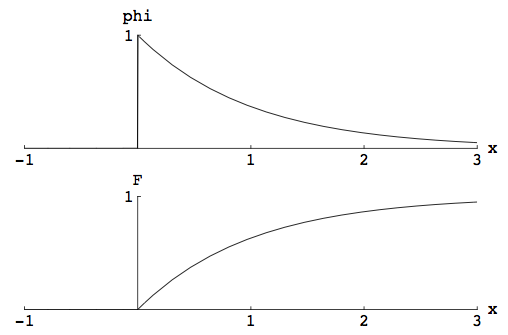
\includegraphics[width=8cm]{./bilder/exponentialverteilung.png}
        \caption{Dichtefunktion (oben) und Verteilungsfunktion (unten) der
        Exponentialverteilung.} 		
		\end{floatingfigure}

		Zur Ermittlung der Dauer von zufälligen Zeitintervallen ohne Gedächnis
		(W'keit, dass X in der nächsten Minute defekt geht = const.). Beispiele :
		\begin{itemize}
          \item Lebensdauer von Atomen beim radioaktiven Zerfall
          \item Lebensdauer von Bauteilen, Maschinen \& Geräten\\(MTBF -
          Mean Time Between Failure = $\frac{1}{\lambda}$)
        \end{itemize}
        
		\underline{Dichtefunktion und Verteilungsfunktion}\\
        $\varphi(x)=\begin{cases}
		\lambda e^{-\lambda x}  & x \geq 0\\
  		0						& x < 0
		\end{cases}$
		
		$F(x)=\begin{cases}
  		1-e^{-\lambda x}  		& x \geq 0\\
  		0	 					& x < 0
		\end{cases}$\\ \\

		\underline{Erwartungswert und Varianz}\\
		$E(X)=\frac{1}{\lambda}$\\
		$var(X)=\frac{1}{\lambda^2}$ \\
		
		
\newpage
	\subsection{Hypergeometrische Verteilung \skript{120}}
	    \begin{floatingfigure}[r]{5.5cm}
        	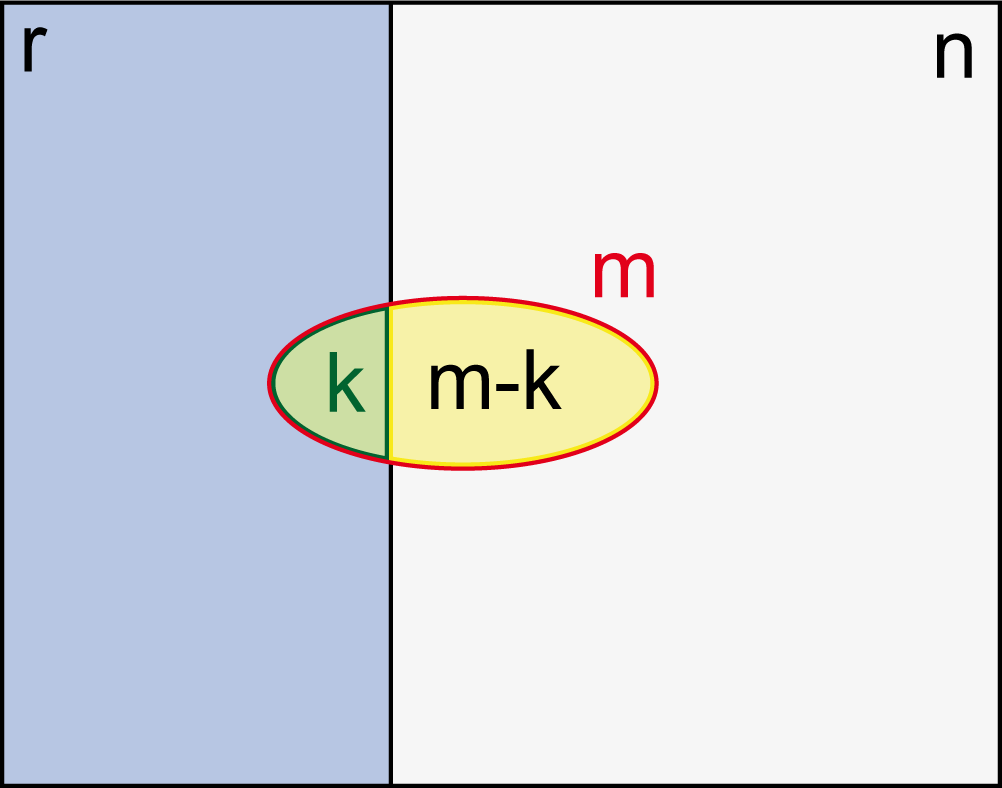
\includegraphics[width=5.5cm]{./bilder/hypergeo.png}
        \end{floatingfigure}
        Ist die Wahrscheinlichkeit dass in einer $m$ Elemente umfassenden 
		Stichprobe aus einer Grundgesamtheit von $n$ Elementen, von denen $r$ eine
		spezielle Eigenschaft besitzen, $k$ Elemente mit der Eigenschaft zu
		finden sind.\\
		\vspace{5mm} 
		$p(k)=P(X=k)=\dfrac{\binom r k \binom{n-r}{m-k}}{\binom n m}$ 
        \hspace{10mm} für $0\leq k \leq r$ und $k \leq n$\\
        Erwartungswert: \hspace{10mm} $E(X)=m \dfrac{r}{n}$\\
        Varianz: \hspace{22mm} $var(X)=m \dfrac{r(n-r)(n-m)}{n^2(n-1)}$ \\
		{\bf Beispiel:} \\
		Lotto, $n=45$ Zahlen, $r=6$ (die gezogenen Zahlen), $m=6$
		(meine Zahlen) \\
		$P(X=4)=P(\text{Ein Vierer})=\dfrac{\binom 6 4 \binom {39}
		2}{\binom {45} 6}=0.001364$	\\

\hrule \hspace{3mm}

	\subsection{Poissonverteilung \skript{128}}
	\begin{multicols}{2}
		\begin{tabular}{ll}
        $P_\lambda(k)=\frac{\lambda^k}{k!}e^{-\lambda}$ & \\
        Erwartungswert:  & $E(X)=\lambda$\\
        Varianz:  & $var(X)=\lambda$ \\
        $\lambda = a \cdot x$ \\
        \end{tabular} \\
         $P(X<k) = \sum_0^k P_\lambda(k)=\sum_0^k \frac{\lambda^k}{k!}e^{-\lambda}$ \\
         $P(X>k) = 1-P(X<k)$ \\
        \columnbreak
        
        {\bf Anwendungsbeispiele:} \\ Für die Häufigkeiten seltener
        Ereignisse. Anzahl Anrufe bei einer Telefonzentrale in einer gewissen
        Periode. Anzahl grosse Versicherungsschäden in einer gewissen Periode.
        Anzahl Jobs, die bei einem Server ankommen. Anzahl Ereignisse in
        einem Zeitintervall. Anzahl Lokomotiven der SBB, die in der nächsten Woche 
        einen Defekt haben. Anzahl der Gewinner mit 4 Richtigen im Lotto.
     \end{multicols}
        

\hrule

		\subsection{Binomialverteilung \skript{125}}
		\begin{tabular}{p{18cm}}
    	Wird angewendet bei einem Experiment mit nur zwei Ausgängen (Ereignis mit W'keit $p$ tritt
    	ein, Ereignis tritt nicht ein). \\
    	Eine Zufallsvariable mit diskreten Werten $k \in \{
    	0,\ldots,n \}$ heisst binomialverteilt zum Parameter $p$, wenn die
        Wahrscheinlichkeit des Wertes $k$ wie folgt ist:
        %\end{tabular}
		%\begin{center}
		$$X = Bi(n; p) = \binom n k p^k(1-p)^{n-k} \qquad \mu = E(X) = p \cdot n \qquad \sigma^2 =
		var(X) = n \cdot p (1-p)$$
		%\end{center}
		%\begin{tabular}{ll} 
		
		$n$: Versuche \hspace{10mm}
		$k$: k-mal erfolgreich \hspace{10mm}
		$p$: Wahrscheinlichkeit\\\\
		
		{\bf Beispiel:} Wie hoch ist die Wahrscheinlichkeit, dass bei 350 Leuten genau
		k $(k\leq 350)$ heute Geburtstag haben?\\
		$P(k)=\binom {350} k \left(\frac{1}{365}\right)^k
		\left(\frac{364}{365}\right)^{350-k}$
		
        \end{tabular}


\hrule
		\subsection{Gleichverteilung}
		\begin{tabular}{p{9cm} p{9cm}}
        %$M_n=\frac{X_1+\ldots+X_n}{n}$ \hspace{10mm} $M_n$: Mittelwert\\
		\textbf{Stetig \skript{93}} 
		& \textbf{Diskret \skript{116}} \\
		Erwartungswert: $E(X)=\frac{a + b}{2}$
		& Erwartungswert: $E(X)=\frac{n + 1}{2}$\\
		Varianz: $var(X)=\frac{(b-a)^2}{12}$
		& Varianz: $var(X)=\frac{n^2-1}{12}$
        \end{tabular}
\vspace{1mm}
\hrule